\chapter{Prezentacja warstwy użytkowej projektu}

Graficzny interfejs użytkownika (GUI) został opracowany z myślą o prostocie obsługi, czytelności i intuicyjnej nawigacji. System udostępnia dwa główne panele: dla użytkownika typu \textbf{pacjent} oraz dla użytkownika typu \textbf{sekretariat}. Poniżej zaprezentowano poszczególne widoki oraz ich funkcjonalność.

\section{Okno powitalne}
To pierwsze okno aplikacji, z którego użytkownik może przejść do logowania lub zakończyć program.

\begin{figure}[H]
\centering
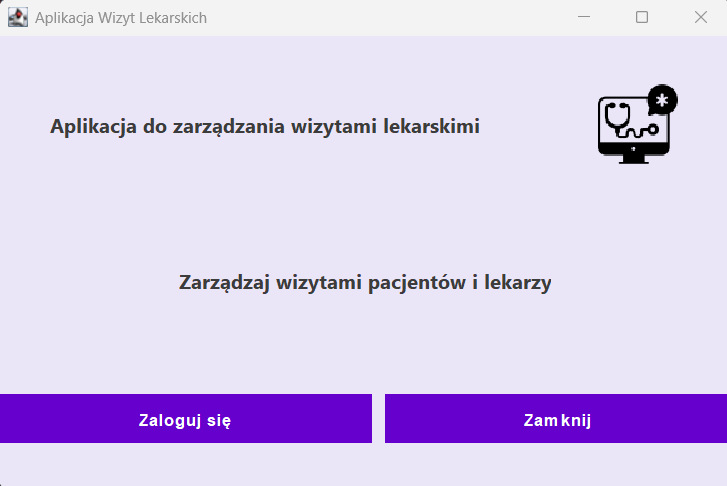
\includegraphics[width=0.7\textwidth]{figures/okno_powitalne.png}
\caption{Okno powitalne aplikacji}
\end{figure}

\section{Panel logowania}
Panel ten zawiera pola do wpisania loginu i hasła oraz przycisk do zalogowania. W przypadku błędnych danych użytkownik otrzymuje stosowny komunikat.

\begin{figure}[H]
\centering
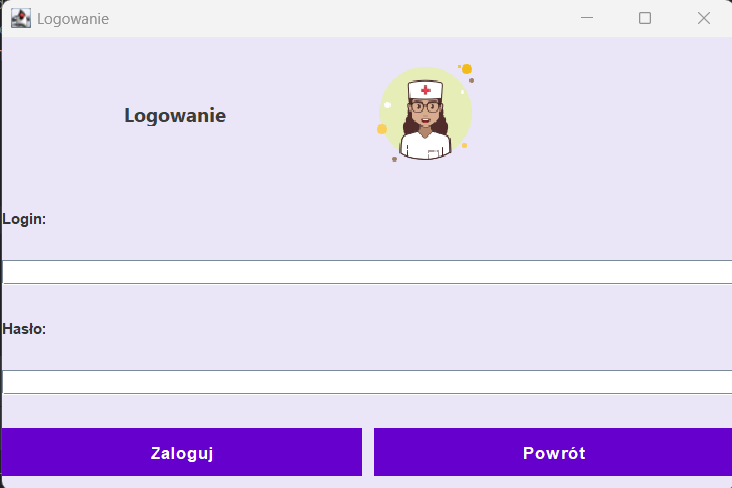
\includegraphics[width=0.7\textwidth]{figures/okno_logowania.png}
\caption{Ekran logowania}
\end{figure}

\section{Panel sekretariatu}
Po zalogowaniu się jako sekretarz użytkownik ma dostęp do głównego panelu zarządzania. Sekretariat może przeglądać, dodawać, edytować oraz usuwać dane pacjentów, lekarzy i wizyt.

\begin{figure}[H]
\centering
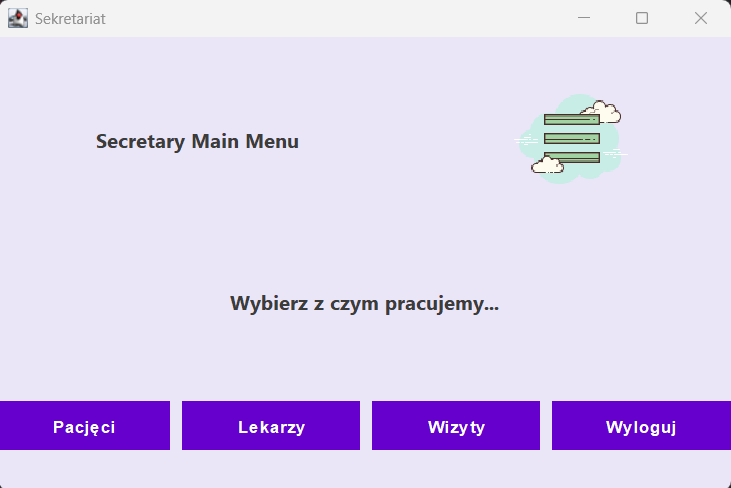
\includegraphics[width=0.75\textwidth]{figures/secretary_main_menu.png}
\caption{Główny panel sekretariatu}
\end{figure}

\section{Zarządzanie lekarzami}
Sekretariat posiada osobne okno do zarządzania lekarzami. W tym widoku możliwe jest przeglądanie listy wszystkich lekarzy oraz wykonywanie operacji CRUD (Dodaj, Edytuj, Usuń).

\begin{figure}[H]
\centering
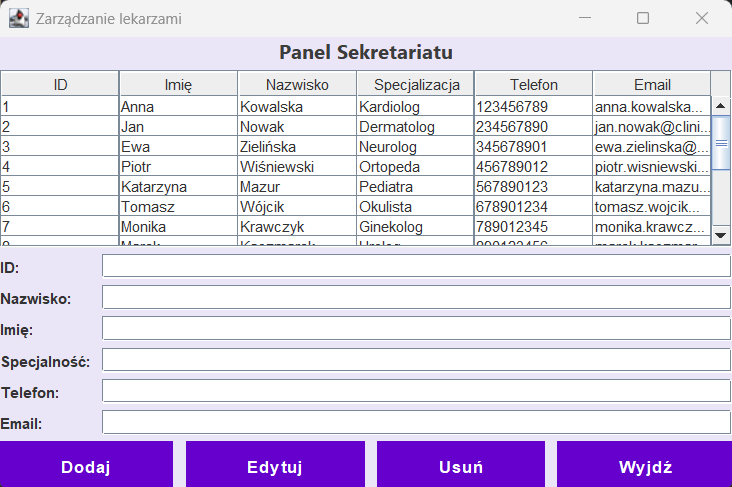
\includegraphics[width=0.75\textwidth]{figures/EditingDoctorsPanel.png}
\caption{Zarządzanie lekarzami – widok sekretariatu}
\end{figure}

\clearpage
\section{Panel pacjenta}
Po zalogowaniu się jako pacjent użytkownik ma dostęp do panelu z opcjami: „Moje dane”, „Moje wizyty”, „Zarezerwuj wizytę” oraz „Wyloguj”.

\begin{figure}[H]
\centering
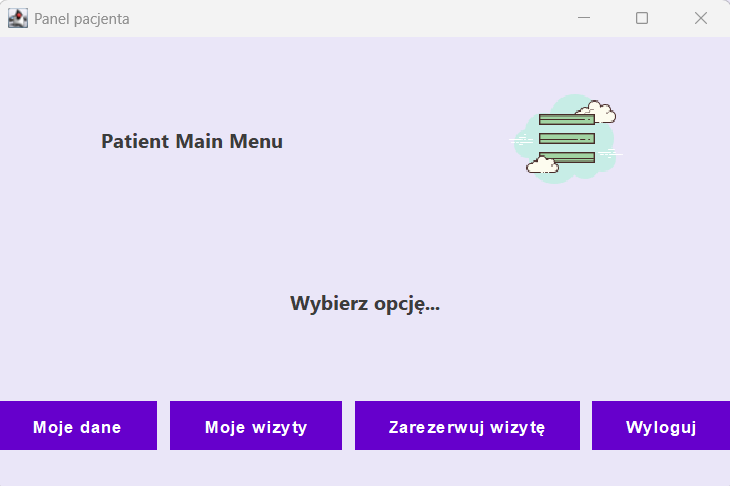
\includegraphics[width=0.75\textwidth]{figures/patient_panel.png}
\caption{Panel główny pacjenta}
\end{figure}


\section{Formularz danych pacjenta}
Panel „Moje dane” umożliwia pacjentowi podgląd danych osobowych, takich jak imię, nazwisko, PESEL, email oraz numer telefonu.

\begin{figure}[H]
\centering
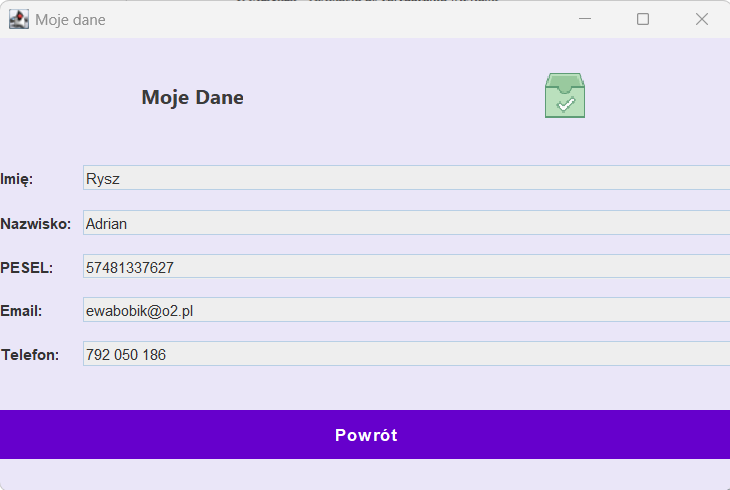
\includegraphics[width=0.7\textwidth]{figures/MyDataPatients.png}
\caption{Widok danych pacjenta}
\end{figure}
\clearpage
\section{Formularz rezerwacji wizyty}
W tym oknie pacjent może zarezerwować wizytę, wybierając lekarza z listy oraz wpisując dokładną datę i godzinę w formacie \texttt{YYYY-MM-DD HH:mm}.

\begin{figure}[H]
\centering
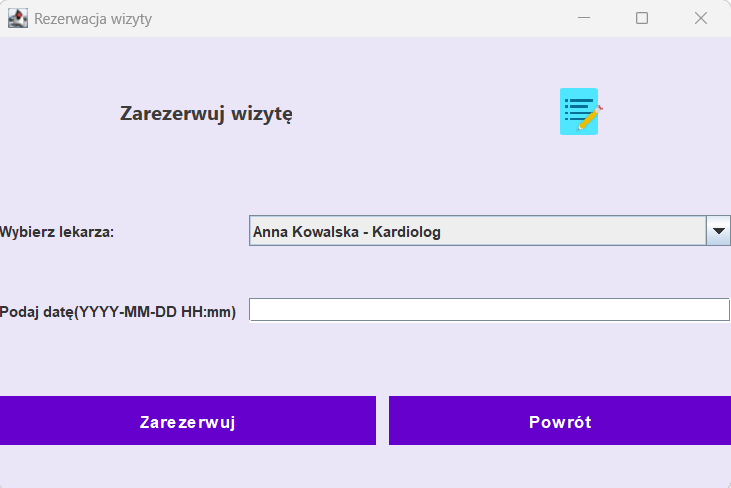
\includegraphics[width=0.7\textwidth]{figures/ReserveVisit.png}
\caption{Formularz rezerwacji wizyty}
\end{figure}

\section{Tabela wizyt}
Widok tabelaryczny wizyt umożliwia przeglądanie istniejących wpisów, filtrowanie oraz odświeżanie zawartości.

\begin{figure}[H]
\centering
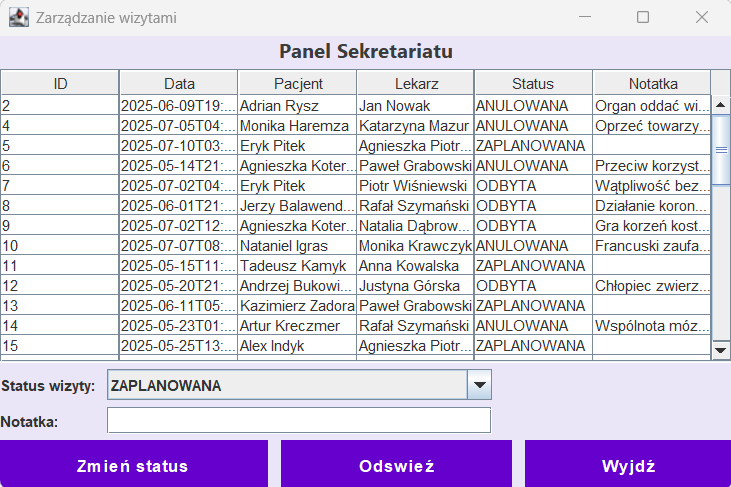
\includegraphics[width=0.7\textwidth]{figures/visit_table.png}
\caption{Tabela wizyt z funkcją odświeżania}
\end{figure}

\clearpage
\section{Tworzenie danych logowania pacjenta}
Podczas dodawania nowego pacjenta możliwe jest także automatyczne tworzenie konta użytkownika z przypisaną rolą.

\begin{figure}[H]
\centering
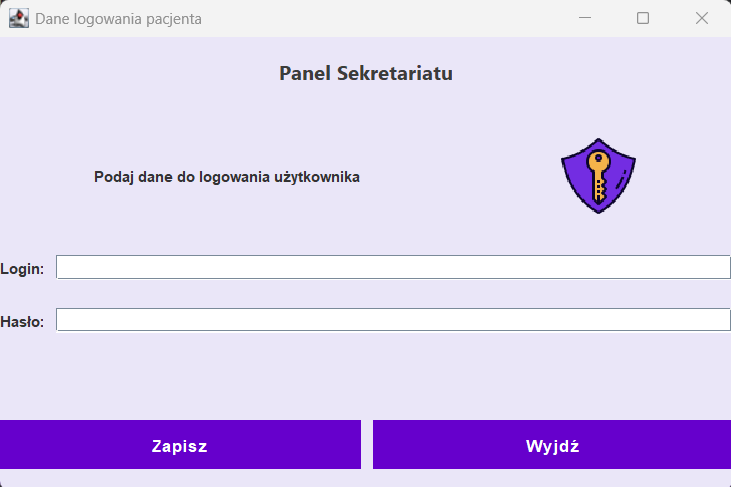
\includegraphics[width=0.7\textwidth]{figures/login_data.png}
\caption{Formularz do tworzenia konta pacjenta}
\end{figure}
